\section{Problem: (2,3)-Bäume}

\subsection{Aufgabenstellung}
Fügen Sie der Reihe nach die Schlüssel 1, 2, 3, 4, 5, 6, 7, 8 in einen leeren 2-3-Baum ein. Löschen Sie anschließend 3 und 6, und fügen Sie die Schlüssel 9 und 10 ein. Zeichnen Sie den 2-3-Baum nach jeder Umstrukturierung (nicht nur am Ende jeder
Einfüge- oder Löschoperation), und markieren Sie die Knoten, wo die 2-3-Baum Eigenschaft verletzt ist. Es reicht, wenn Sie die Gestalt des 2-3-Baums und die Schlüssel in den Blättern zeichnen; die Schlüssel in den inneren Knoten brauchen Sie nicht anzugeben.

\subsection{Gegeben}

Ein (2,3)-Baum hat folgende Grenzen:
\begin{itemize}
	\item min children: 2, max children: 3
	\item min entries: 1, max entries: 2
	\item Leerer Baum:
	\begin{itemize}
		\item Schlüssel(Einfügen): 1, 2, 3, 4, 5, 6, 7, 8
		\item Schlüssel(Löschen): 3, 6
		\item Schlüssel(Einfügen): 9, 10
	\end{itemize}
\end{itemize}

\subsection{Lösung}

\begin{multicols}{2}
	
	\begin{enumerate}
		
		\item insert(1):
		
		\begin{tikzpicture}[scale=0.5,
			level 1/.style={sibling distance=40mm},
			level 2/.style={sibling distance=20mm},
			level 3/.style={sibling distance=20mm},
			level 4/.style={sibling distance=20mm}]
			\node{$[]^1$};
		\end{tikzpicture}

		\begin{tikzpicture}[scale=0.5,
			level 1/.style={sibling distance=40mm},
			level 2/.style={sibling distance=20mm},
			level 3/.style={sibling distance=20mm},
			level 4/.style={sibling distance=20mm}]
			\node{$[1]$};
		\end{tikzpicture}
		
		\item insert(2):
		
		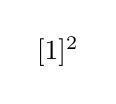
\begin{tikzpicture}[scale=0.5,
			level 1/.style={sibling distance=40mm},
			level 2/.style={sibling distance=20mm},
			level 3/.style={sibling distance=20mm},
			level 4/.style={sibling distance=20mm}]
			\node{$[1]^2$};
		\end{tikzpicture}
		
		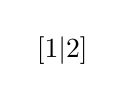
\begin{tikzpicture}[scale=0.5,
			level 1/.style={sibling distance=40mm},
			level 2/.style={sibling distance=20mm},
			level 3/.style={sibling distance=20mm},
			level 4/.style={sibling distance=20mm}]
			\node{$[1|2]$};
		\end{tikzpicture}
		
		\item insert(3):
		
		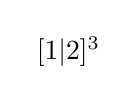
\begin{tikzpicture}[scale=0.5,
			level 1/.style={sibling distance=40mm},
			level 2/.style={sibling distance=20mm},
			level 3/.style={sibling distance=20mm},
			level 4/.style={sibling distance=20mm}]
			\node{$[1|2]^3$};
		\end{tikzpicture}

		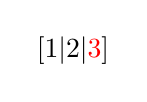
\begin{tikzpicture}[scale=0.5,
			level 1/.style={sibling distance=40mm},
			level 2/.style={sibling distance=20mm},
			level 3/.style={sibling distance=20mm},
			level 4/.style={sibling distance=20mm}]
			\node{$[1|2|\textcolor{red}{3}]$};
		\end{tikzpicture}
		\begin{itemize}
			\item Maximaleinträge in der Wurzel verletzt $\rightarrow$ Split
			\item Suche die Mitte $m = \lfloor \frac{b+1}{2} \rfloor$
			\item $m = \lfloor \frac{3+1}{2} \rfloor$
			\item $m = 2$ $\rightarrow$ Eintrag 2 = 2 wird zur neuen Wurzel!
		\end{itemize}
		
		\begin{tikzpicture}[scale=0.5,
			level 1/.style={sibling distance=40mm},
			level 2/.style={sibling distance=20mm},
			level 3/.style={sibling distance=20mm},
			level 4/.style={sibling distance=20mm}]
			\node{$[2]$}
				child{ node{$[1]$}}
				child[missing]
				child{ node{$[3]$}};
		\end{tikzpicture}

$\Rightarrow$ $(a,b)$-Baum Eigenschaften wieder hergestellt!

		\item insert(4):

		\begin{tikzpicture}[scale=0.5,
			level 1/.style={sibling distance=40mm},
			level 2/.style={sibling distance=20mm},
			level 3/.style={sibling distance=20mm},
			level 4/.style={sibling distance=20mm}]
			\node{$[2]^4$}
			child{ node{$[1]$}}
			child[missing]
			child{ node{$[3]^4$}};
		\end{tikzpicture}
		
		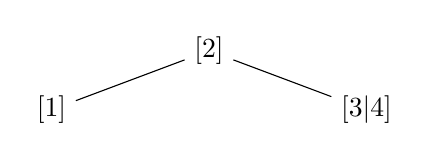
\begin{tikzpicture}[scale=0.5,
			level 1/.style={sibling distance=40mm},
			level 2/.style={sibling distance=20mm},
			level 3/.style={sibling distance=20mm},
			level 4/.style={sibling distance=20mm}]
			\node{$[2]$}
			child{ node{$[1]$}}
			child[missing]
			child{ node{$[3|4]$}};
		\end{tikzpicture}
		
		\item insert(5):
		
		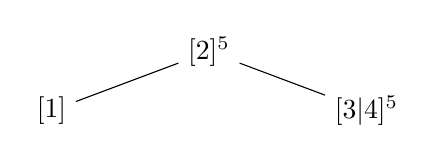
\begin{tikzpicture}[scale=0.5,
			level 1/.style={sibling distance=40mm},
			level 2/.style={sibling distance=20mm},
			level 3/.style={sibling distance=20mm},
			level 4/.style={sibling distance=20mm}]
			\node{$[2]^5$}
			child{ node{$[1]$}}
			child[missing]
			child{ node{$[3|4]^5$}};
		\end{tikzpicture}

		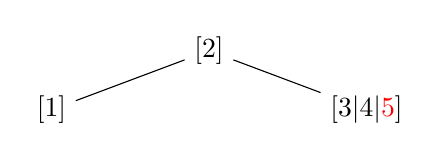
\begin{tikzpicture}[scale=0.5,
			level 1/.style={sibling distance=40mm},
			level 2/.style={sibling distance=20mm},
			level 3/.style={sibling distance=20mm},
			level 4/.style={sibling distance=20mm}]
			\node{$[2]$}
			child{ node{$[1]$}}
			child[missing]
			child{ node{$[3|4|\textcolor{red}{5}]$}};
		\end{tikzpicture}
		\begin{itemize}
			\item Maximaleinträge in dem Blatt $[3|4|5]$ verletzt $\rightarrow$ Split
			\item $m = 2$ $\rightarrow$ Eintrag 2 = 4 wird zur Wurzel geschoben und Blatt aufgeteilt!
		\end{itemize}

		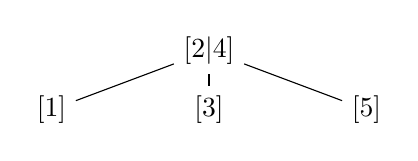
\begin{tikzpicture}[scale=0.5,
			level 1/.style={sibling distance=40mm},
			level 2/.style={sibling distance=20mm},
			level 3/.style={sibling distance=20mm},
			level 4/.style={sibling distance=20mm}]
			\node{$[2|4]$}
			child{ node{$[1]$}}
			child{ node{$[3]$}}
			child{ node{$[5]$}};
		\end{tikzpicture}
		
		$\Rightarrow$ $(a,b)$-Baum Eigenschaften wieder hergestellt!

		\item insert(6):
		
		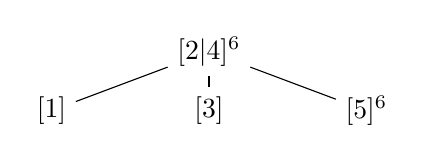
\begin{tikzpicture}[scale=0.5,
			level 1/.style={sibling distance=40mm},
			level 2/.style={sibling distance=20mm},
			level 3/.style={sibling distance=20mm},
			level 4/.style={sibling distance=20mm}]
			\node{$[2|4]^6$}
			child{ node{$[1]$}}
			child{ node{$[3]$}}
			child{ node{$[5]^6$}};
		\end{tikzpicture}

		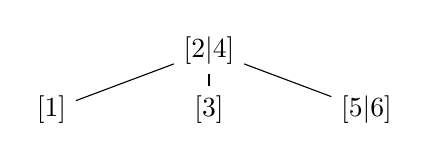
\begin{tikzpicture}[scale=0.5,
			level 1/.style={sibling distance=40mm},
			level 2/.style={sibling distance=20mm},
			level 3/.style={sibling distance=20mm},
			level 4/.style={sibling distance=20mm}]
			\node{$[2|4]$}
			child{ node{$[1]$}}
			child{ node{$[3]$}}
			child{ node{$[5|6]$}};
		\end{tikzpicture}
		
		\item insert(7):
		
		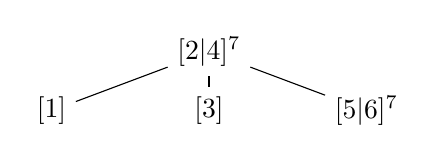
\begin{tikzpicture}[scale=0.5,
			level 1/.style={sibling distance=40mm},
			level 2/.style={sibling distance=20mm},
			level 3/.style={sibling distance=20mm},
			level 4/.style={sibling distance=20mm}]
			\node{$[2|4]^7$}
			child{ node{$[1]$}}
			child{ node{$[3]$}}
			child{ node{$[5|6]^7$}};
		\end{tikzpicture}

		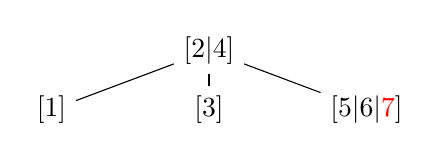
\begin{tikzpicture}[scale=0.5,
			level 1/.style={sibling distance=40mm},
			level 2/.style={sibling distance=20mm},
			level 3/.style={sibling distance=20mm},
			level 4/.style={sibling distance=20mm}]
			\node{$[2|4]$}
			child{ node{$[1]$}}
			child{ node{$[3]$}}
			child{ node{$[5|6|\textcolor{red}{7}]$}};
		\end{tikzpicture}
			\begin{itemize}
			\item Maximaleinträge in dem Blatt $[5|6|7]$ verletzt $\rightarrow$ Split
			\item $m = 2$ $\rightarrow$ Eintrag 2 = 6 wird zur Wurzel geschoben und Blatt aufgeteilt!
		\end{itemize}
		
		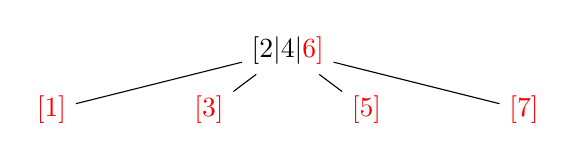
\begin{tikzpicture}[scale=0.5,
			level 1/.style={sibling distance=40mm},
			level 2/.style={sibling distance=20mm},
			level 3/.style={sibling distance=20mm},
			level 4/.style={sibling distance=20mm}]
			\node{$[2|4|\textcolor{red}{6]}$}
			child{ node{$\textcolor{red}{[1]}$}}
			child{ node{$\textcolor{red}{[3]}$}}
			child{ node{$\textcolor{red}{[5]}$}}
			child{ node{$\textcolor{red}{[7]}$}};
		\end{tikzpicture}
		\begin{itemize}
			\item Maximaleinträge in dem Wurzel überschritten \& die Maxiamle anzahl der Kinder verletzt $\rightarrow$ Split der Wurzel
			\item $m = 2$ $\rightarrow$ Eintrag 2 = 4 wird zur Wurzel geschoben und Blatt aufgeteilt!
		\end{itemize}
		
		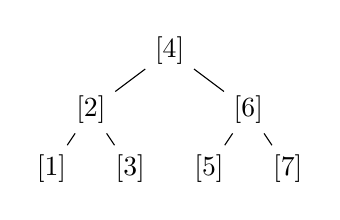
\begin{tikzpicture}[scale=0.5,
			level 1/.style={sibling distance=40mm},
			level 2/.style={sibling distance=20mm},
			level 3/.style={sibling distance=20mm},
			level 4/.style={sibling distance=20mm}]
			
			\node{$[4]$}
			child { node{$[2]$}
				child { node{$[1]$} }
				child { node{$[3]$} }
			}
			child { node{$[6]$}
				child { node{$[5]$} }
				child { node{$[7]$} } };
		\end{tikzpicture}
		
		$\Rightarrow$ $(a,b)$-Baum Eigenschaft wiederhergestellt


		\item insert(8):
		
		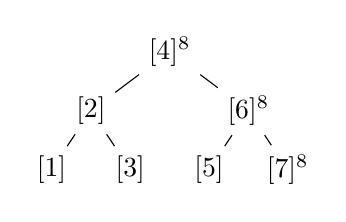
\begin{tikzpicture}[scale=0.5,
			level 1/.style={sibling distance=40mm},
			level 2/.style={sibling distance=20mm},
			level 3/.style={sibling distance=20mm},
			level 4/.style={sibling distance=20mm}]
			
			\node{$[4]^8$}
			child { node{$[2]$}
				child { node{$[1]$} }
				child { node{$[3]$} }
			}
			child { node{$[6]^8$}
				child { node{$[5]$} }
				child { node{$[7]^8$} } };
		\end{tikzpicture}
		
		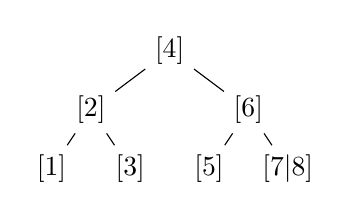
\begin{tikzpicture}[scale=0.5,
			level 1/.style={sibling distance=40mm},
			level 2/.style={sibling distance=20mm},
			level 3/.style={sibling distance=20mm},
			level 4/.style={sibling distance=20mm}]
			
			\node{$[4]$}
			child { node{$[2]$}
				child { node{$[1]$} }
				child { node{$[3]$} }
			}
			child { node{$[6]$}
				child { node{$[5]$} }
				child { node{$[7|8]$} } };
		\end{tikzpicture}
		
		\item remove(3):
		
		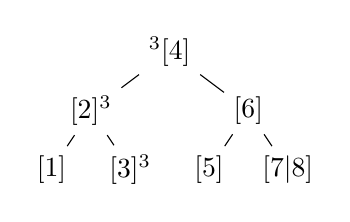
\begin{tikzpicture}[scale=0.5,
			level 1/.style={sibling distance=40mm},
			level 2/.style={sibling distance=20mm},
			level 3/.style={sibling distance=20mm},
			level 4/.style={sibling distance=20mm}]
			
			\node{$^3[4]$}
			child { node{$[2]^3$}
				child { node{$[1]$} }
				child { node{$[3]^3$} }
			}
			child { node{$[6]$}
				child { node{$[5]$} }
				child { node{$[7|8]$} } };
		\end{tikzpicture}
		
		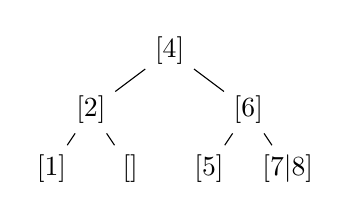
\begin{tikzpicture}[scale=0.5,
			level 1/.style={sibling distance=40mm},
			level 2/.style={sibling distance=20mm},
			level 3/.style={sibling distance=20mm},
			level 4/.style={sibling distance=20mm}]
			
			\node{$[4]$}
			child { node{$[2]$}
				child { node{$[1]$} }
				child { node{$[]$} }
			}
			child { node{$[6]$}
				child { node{$[5]$} }
				child { node{$[7|8]$} } };
		\end{tikzpicture}
		
		$\rightarrow$ Eintrag 3 wurde entfern, wir haben nun ein verletzung der min. Einträge in einem Blatt\\
		$\rightarrow$ alle direkten Nachbarn haben $a-1$ Einträge, also Verschmeltzen von Konten!
		
		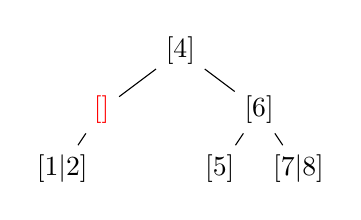
\begin{tikzpicture}[scale=0.5,
			level 1/.style={sibling distance=40mm},
			level 2/.style={sibling distance=20mm},
			level 3/.style={sibling distance=20mm},
			level 4/.style={sibling distance=20mm}]
			
			\node{$[4]$}
			child { node{$\textcolor{red}{[]}$}
				child { node{$[1|2]$} }
				child[missing]
			}
			child { node{$[6]$}
				child { node{$[5]$} }
				child { node{$[7|8]$} } };
		\end{tikzpicture}
		
		$\rightarrow$ Der Elternknoten hat nun keine Kinder mehr und direkter Nachbar hat nur $a-1$ Einträge, wir klauen aus dem Elternknoten wieder ein Eintrag und Verschmelzen die Knoten!
		
		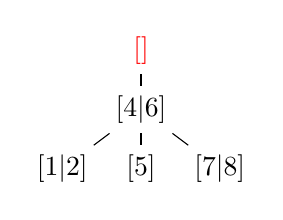
\begin{tikzpicture}[scale=0.5,
			level 1/.style={sibling distance=40mm},
			level 2/.style={sibling distance=20mm},
			level 3/.style={sibling distance=20mm},
			level 4/.style={sibling distance=20mm}]
			
			\node{$\textcolor{red}{[]}$}
			child { node{$[4|6]$}
				child { node{$[1|2]$} }
				child { node{$[5]$} }
				child { node{$[7|8]$} }
			};
		\end{tikzpicture}

		$\rightarrow$ Speziallfall, die Wurzel ist nun leer, wir können Sie einfach löschen und eine Neue Wurzel erschaffen.
		
		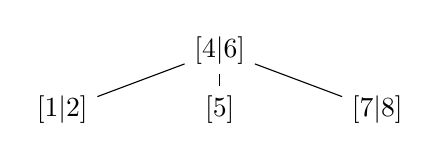
\begin{tikzpicture}[scale=0.5,
			level 1/.style={sibling distance=40mm},
			level 2/.style={sibling distance=20mm},
			level 3/.style={sibling distance=20mm},
			level 4/.style={sibling distance=20mm}]
			
			\node{$[4|6]$}
			child { node{$[1|2]$} }
			child { node{ $[5]$ } }
			child { node{ $[7|8]$ } 
			};
		\end{tikzpicture}
		
		$\rightarrow$$(a,b)$-Baum Eigenschaften wieder Hergestellt!
		
		\item \textbf{remove(6):}
		
		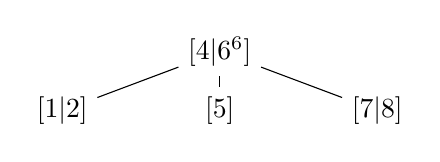
\begin{tikzpicture}[scale=0.5,
			level 1/.style={sibling distance=40mm},
			level 2/.style={sibling distance=20mm},
			level 3/.style={sibling distance=20mm},
			level 4/.style={sibling distance=20mm}]
			
			\node{$[4|6^6]$}
			child { node{$[1|2]$} }
			child { node{ $[5]$ } }
			child { node{ $[7|8]$ } 
			};
		\end{tikzpicture}

		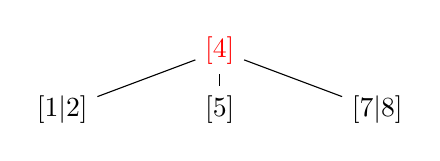
\begin{tikzpicture}[scale=0.5,
			level 1/.style={sibling distance=40mm},
			level 2/.style={sibling distance=20mm},
			level 3/.style={sibling distance=20mm},
			level 4/.style={sibling distance=20mm}]
			
			\node{$\textcolor{red}{[4]}$}
			child { node{$[1|2]$} }
			child { node{ $[5]$ } }
			child { node{ $[7|8]$ } 
			};
		\end{tikzpicture}
		
		$\rightarrow$ Die Wurzel hat nun zu wenige Einträge um die Kinderstruktur aufrecht zu erhalten
		$\rightarrow$ Wir suchen nun den Vorgänger von 6, also 5 und ersetzten 6 durch die 5!
		
		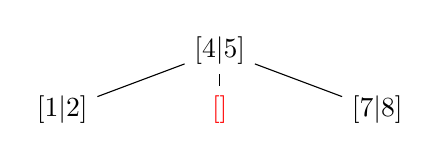
\begin{tikzpicture}[scale=0.5,
			level 1/.style={sibling distance=40mm},
			level 2/.style={sibling distance=20mm},
			level 3/.style={sibling distance=20mm},
			level 4/.style={sibling distance=20mm}]
			
			\node{$[4|5]$}
			child { node{$[1|2]$} }
			child { node{ $\textcolor{red}{[]}$ } }
			child { node{ $[7|8]$ } 
			};
		\end{tikzpicture}
		
		$\rightarrow$ Nun ist die Wurzel wieder Ordentlich, leider ist ein Blatt nun leer, wir leihen uns nun ein Eintrag aus einem linken teilbaum aus		

		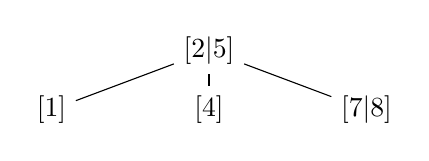
\begin{tikzpicture}[scale=0.5,
			level 1/.style={sibling distance=40mm},
			level 2/.style={sibling distance=20mm},
			level 3/.style={sibling distance=20mm},
			level 4/.style={sibling distance=20mm}]
			
			\node{$[2|5]$}
			child { node{$[1]$} }
			child { node{ $[4]$ } }
			child { node{ $[7|8]$ } 
			};
		\end{tikzpicture}
		
		$\rightarrow(a,b)$-Baum Eigenschaft wieder Hergestellt!

		\item \textbf{insert(9):}
		
		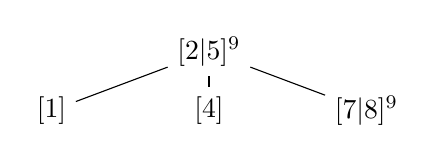
\begin{tikzpicture}[scale=0.5,
			level 1/.style={sibling distance=40mm},
			level 2/.style={sibling distance=20mm},
			level 3/.style={sibling distance=20mm},
			level 4/.style={sibling distance=20mm}]
			
			\node{$[2|5]^9$}
			child { node{$[1]$} }
			child { node{ $[4]$ } }
			child { node{ $[7|8]^9$ } 
			};
		\end{tikzpicture}
		
		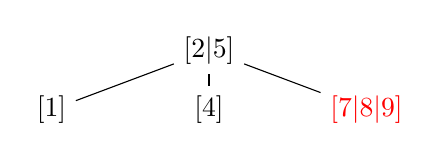
\begin{tikzpicture}[scale=0.5,
			level 1/.style={sibling distance=40mm},
			level 2/.style={sibling distance=20mm},
			level 3/.style={sibling distance=20mm},
			level 4/.style={sibling distance=20mm}]
			
			\node{$[2|5]$}
			child { node{$[1]$} }
			child { node{ $[4]$ } }
			child { node{ $\textcolor{red}{[7|8|9]}$ } 
			};
		\end{tikzpicture}
		
		\begin{itemize}
			\item Maximaleinträge in dem Wurzel überschritten \& die Maxiamle anzahl der Kinder verletzt $\rightarrow$ Split der Wurzel
			\item $m = 2$ $\rightarrow$ Eintrag 2 = 8 wird zur Wurzel geschoben und Blatt aufgeteilt!
		\end{itemize}
		
		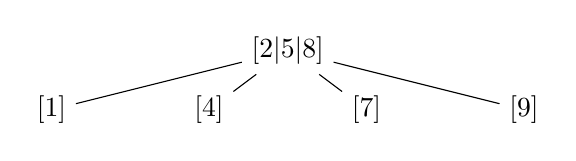
\begin{tikzpicture}[scale=0.5,
			level 1/.style={sibling distance=40mm},
			level 2/.style={sibling distance=20mm},
			level 3/.style={sibling distance=20mm},
			level 4/.style={sibling distance=20mm}]
			
			\node{$[2|5|8]$}
			child { node{$[1]$} }
			child { node{ $[4]$ } }
			child { node{ $[7]$ } }
			child { node{ $[9]$ } 
			};
		\end{tikzpicture}
		
		$\rightarrow$ Die Wurzle hat nun zuviele Einträge, bzw. haben wir zu viele Kinder
		$\rightarrow$ Wir spliten die Wurzel!
		
		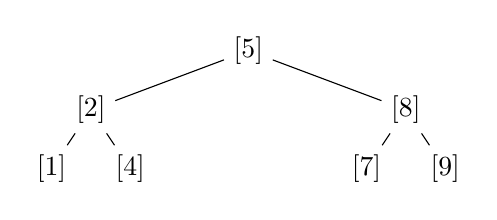
\begin{tikzpicture}[scale=0.5,
			level 1/.style={sibling distance=40mm},
			level 2/.style={sibling distance=20mm},
			level 3/.style={sibling distance=20mm},
			level 4/.style={sibling distance=20mm}]
			
			\node{$[5]$}
			child { node{$[2]$} 
				child{ node{ $[1]$ } }
				child{ node{ $[4]$ } }
				}
			child[missing]
			child { node{ $[8]$ } 
				child{ node{ $[7]$ } }
				child{ node{ $[9]$ } }
				};
		\end{tikzpicture}
		
		$\rightarrow$$(a,b)$-Baum Eigenschaft wiederhergestellt!
		
		\item \textbf{insert(10):}
		
		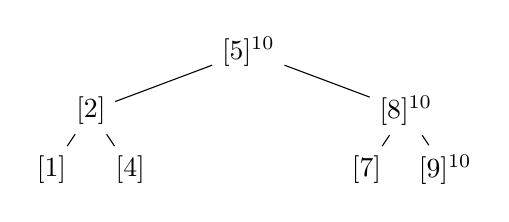
\begin{tikzpicture}[scale=0.5,
			level 1/.style={sibling distance=40mm},
			level 2/.style={sibling distance=20mm},
			level 3/.style={sibling distance=20mm},
			level 4/.style={sibling distance=20mm}]
			
			\node{$[5]^{10}$}
			child { node{$[2]$} 
				child{ node{ $[1]$ } }
				child{ node{ $[4]$ } }
			}
			child[missing]
			child { node{ $[8]^{10}$ } 
				child{ node{ $[7]$ } }
				child{ node{ $[9]^{10}$ } }
			};
		\end{tikzpicture}
		
		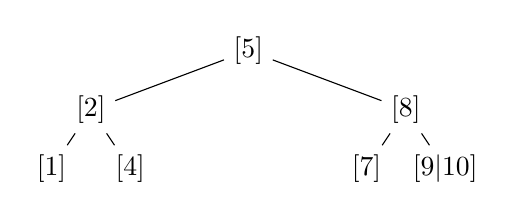
\begin{tikzpicture}[scale=0.5,
			level 1/.style={sibling distance=40mm},
			level 2/.style={sibling distance=20mm},
			level 3/.style={sibling distance=20mm},
			level 4/.style={sibling distance=20mm}]
			
			\node{$[5]$}
			child { node{$[2]$} 
				child{ node{ $[1]$ } }
				child{ node{ $[4]$ } }
			}
			child[missing]
			child { node{ $[8]$ } 
				child{ node{ $[7]$ } }
				child{ node{ $[9|10]$ } }
			};
		\end{tikzpicture}

	\end{enumerate}
\end{multicols}